
\section{Summary Statistics}
\label{sec:appendixsumstat}

Table~\ref{tab:summarytab1} and Table~\ref{tab:summarytab2} display univariate summary statistics from the primary dataset. We display the mean, interquartile range, and the range (as defined by the maximum value minus the minimum value) for the unadjusted dataset (sigma\_zero), the preferred adjustment (sigma\_uu\_i), and the secondary adjustment (sigma\_uu\_avg). We see that in general the covariate adjustments reduce the variability in the data. However, we also see that the range sometimes increases drastically, particularly for the untreated dataset. Table~\ref{tab:extreme1} displays the overall number of CPUMAs whose adjusted values fall outside of the range of the unadjusted data. Note that for our ETT estimates, we only use the adjustments on the treatment data, while we use both for the OATE estimates. 
We also calculate these adjustments when leaving out each state one at a time from the primary dataset to calculate our secondary variance estimates; these results are available on request. 

\begin{table}[ht]
\centering
    \caption{Univariate summary statistics (1)}
    \label{tab:summarytab1}
\begin{tabular}{rllll}
  \toprule
Treatment & Variable & sigma\_zero & sigma\_uu\_i & sigma\_uu\_avg \\ 
  \midrule
0 & age\_cat2\_19\_29\_pct & (24.8, 5.5, 48.7) & (24.8, 5.4, 47.5) & (24.8, 5.4, 47.8) \\ 
  1 & age\_cat2\_19\_29\_pct & (24.5, 6, 30.9) & (24.5, 5.9, 29) & (24.5, 5.9, 29) \\ 
  0 & age\_cat2\_30\_39\_pct & (20.6, 2.6, 18.4) & (20.6, 2.5, 17.3) & (20.6, 2.5, 17.2) \\ 
  1 & age\_cat2\_30\_39\_pct & (20.9, 3.4, 20.9) & (20.9, 3.1, 19.1) & (20.9, 3.2, 19.4) \\ 
  0 & age\_cat2\_40\_49\_pct & (22, 2.5, 19.5) & (22, 2.4, 33.3) & (22, 2.3, 18.5) \\ 
  1 & age\_cat2\_40\_49\_pct & (22.2, 2.5, 15.4) & (22.2, 2.3, 13.8) & (22.2, 2.3, 13.8) \\ 
  0 & avg\_adult\_hh\_ratio & (139.7, 18.7, 156.8) & (139.7, 18.9, 153.7) & (139.7, 18.9, 154.2) \\ 
  1 & avg\_adult\_hh\_ratio & (150.8, 27.1, 174.3) & (150.8, 27, 173.8) & (150.8, 27.1, 173.3) \\ 
  0 & citizenship\_pct & (93.6, 5.9, 39.8) & (93.6, 5.9, 39.7) & (93.6, 5.9, 39.3) \\ 
  1 & citizenship\_pct & (90, 11.8, 57.1) & (90, 11.8, 55.4) & (90, 11.7, 55.7) \\ 
  0 & disability\_pct & (11.9, 5, 22.1) & (11.9, 4.8, 21.1) & (11.9, 4.8, 20.7) \\ 
  1 & disability\_pct & (10.5, 5.3, 28.6) & (10.4, 5.3, 26.7) & (10.5, 5.4, 27.2) \\ 
  0 & educ\_hs\_degree\_pct & (29.6, 8.8, 42.7) & (29.6, 8.8, 40.7) & (29.6, 8.8, 41.2) \\ 
  1 & educ\_hs\_degree\_pct & (26.3, 10.6, 43.2) & (26.3, 10.5, 41.8) & (26.3, 10.6, 41.9) \\ 
  0 & educ\_less\_than\_hs\_pct & (11.8, 7.1, 30) & (11.8, 6.9, 30.2) & (11.8, 7, 30.2) \\ 
  1 & educ\_less\_than\_hs\_pct & (11.4, 7.6, 45.3) & (11.4, 7.4, 45) & (11.4, 7.3, 44.6) \\ 
  0 & educ\_some\_college\_pct & (33.8, 5.6, 42.9) & (33.8, 5.1, 45.7) & (33.8, 5.1, 42.3) \\ 
  1 & educ\_some\_college\_pct & (33.5, 7.8, 34.2) & (33.5, 7.4, 32.8) & (33.5, 7.4, 32.9) \\ 
  0 & female\_pct & (50.5, 1.6, 15.8) & (50.5, 1.5, 14.9) & (50.5, 1.5, 15.1) \\ 
  1 & female\_pct & (50.1, 1.6, 15.4) & (50.1, 1.4, 14.2) & (50.1, 1.5, 14.2) \\ 
  0 & foreign\_born\_pct & (10.5, 8.8, 63.2) & (10.5, 8.9, 62.9) & (10.5, 8.9, 62.7) \\ 
  1 & foreign\_born\_pct & (18, 22.2, 76) & (18, 22.2, 75.2) & (18, 22.2, 75.4) \\ 
  0 & hins\_unins\_pct\_2011 & (22.7, 10.5, 51.4) & (22.3, 10, 757.8) & (22.7, 9.2, 50.1) \\ 
  1 & hins\_unins\_pct\_2011 & (19.6, 11.2, 59) & (19.6, 10.8, 51.8) & (19.6, 10.8, 52.4) \\ 
  0 & hins\_unins\_pct\_2012 & (22.4, 9.3, 49.5) & (22.8, 9.4, 468.8) & (22.4, 9.2, 47.8) \\ 
  1 & hins\_unins\_pct\_2012 & (19.4, 9.8, 50.6) & (19.4, 10, 49.7) & (19.4, 10.1, 50.1) \\ 
  0 & hins\_unins\_pct\_2013 & (22, 10.1, 50.1) & (22.3, 9.4, 323.6) & (22, 9.3, 49.2) \\ 
  1 & hins\_unins\_pct\_2013 & (19, 11.1, 49.9) & (19, 10.2, 48.1) & (19, 10.4, 48.6) \\ 
  0 & hispanic\_pct & (11.4, 10.2, 93.9) & (11.5, 10.2, 93.8) & (11.4, 10.2, 93.8) \\ 
  1 & hispanic\_pct & (15.8, 17.7, 97.2) & (15.8, 17.7, 97) & (15.8, 17.7, 97) \\ 
  0 & inc\_pov2\_138\_pct & (22, 8.8, 42.8) & (22, 8.8, 41) & (22, 8.7, 41.8) \\ 
  1 & inc\_pov2\_138\_pct & (19.9, 11.9, 45.6) & (19.9, 11.7, 44.8) & (19.9, 11.7, 43.9) \\ 
  0 & inc\_pov2\_139\_299\_pct & (27.4, 5.1, 27.9) & (27.2, 4.9, 206.1) & (27.4, 4.8, 26.7) \\ 
  1 & inc\_pov2\_139\_299\_pct & (24.9, 8.4, 34.2) & (24.9, 7.8, 34.2) & (24.9, 7.8, 34.1) \\ 
  0 & inc\_pov2\_300\_499\_pct & (24.2, 4.8, 21) & (24.4, 4.8, 317.6) & (24.2, 4.5, 18.4) \\ 
  1 & inc\_pov2\_300\_499\_pct & (23.6, 5.5, 23) & (23.6, 4.9, 22.2) & (23.6, 4.8, 22.2) \\ 
  0 & inc\_pov2\_500\_plus\_pct & (23.7, 9.9, 51.9) & (23.6, 9.8, 118.8) & (23.7, 9.7, 52.1) \\ 
  1 & inc\_pov2\_500\_plus\_pct & (29.3, 18.4, 69.1) & (29.3, 18.5, 68) & (29.3, 18.4, 68) \\ 
  0 & married\_pct & (51.5, 9.1, 59.7) & (51.6, 8.9, 75.5) & (51.5, 9.1, 59.5) \\ 
  1 & married\_pct & (50.7, 9.4, 45.1) & (50.8, 9, 44.2) & (50.7, 9.1, 44.3) \\ 
  0 & missing\_children\_pct & (13.7, 7.4, 36.2) & (13.8, 7.3, 36.2) & (13.7, 7.3, 35.6) \\ 
  1 & missing\_children\_pct & (10.5, 6.6, 41) & (10.5, 6.6, 40.8) & (10.5, 6.6, 40.5) \\ 
  0 & one\_child\_pct & (10.4, 2.5, 13) & (10.3, 2.1, 159) & (10.4, 2.1, 12.3) \\ 
  1 & one\_child\_pct & (11.1, 3.1, 14.3) & (11.1, 2.8, 12.3) & (11.1, 2.9, 12.5) \\ 
  0 & pop\_growth & (100.3, 1.7, 14.3) & (100.1, 1.2, 267.3) & (100.3, 1, 5) \\ 
  1 & pop\_growth & (100.3, 1.9, 13.7) & (100.3, 1.2, 6.2) & (100.3, 1.2, 6.5) \\ 
  0 & race\_white\_pct & (77.8, 22.2, 90.5) & (77.8, 22.1, 90.2) & (77.8, 22.1, 90.4) \\ 
  1 & race\_white\_pct & (73.9, 25.4, 91.9) & (73.9, 25.5, 91.8) & (73.9, 25.5, 91.8) \\ 
  0 & repub\_gov & (95.9, 0, 100) & (95.9, 0, 100) & (95.9, 0, 100) \\ 
  1 & repub\_gov & (30.9, 100, 100) & (30.9, 100, 100) & (30.9, 100, 100) \\
  0 & repub\_lower\_control & (98.8, 0, 100) & (98.8, 0, 100) & (98.8, 0, 100) \\ 
  1 & repub\_lower\_control & (23.9, 0, 100) & (23.9, 0, 100) & (23.9, 0, 100) \\ 
  0 & repub\_total\_control & (94.7, 0, 100) & (94.7, 0, 100) & (94.7, 0, 100) \\ 
  1 & repub\_total\_control & (21, 0, 100) & (21, 0, 100) & (21, 0, 100) \\ 
   \bottomrule
\end{tabular}
\end{table}

\begin{table}[ht]
\centering
    \caption{Univariate summary statistics (2)}
    \label{tab:summarytab2}
\begin{tabular}{rllll}
  \hline
Treat & Variable & sigma\_zero & sigma\_uu\_avg & sigma\_uu\_i \\ 
  \hline
  0 & student\_pct & (11.5, 3.9, 41) & (11.5, 3.9, 53.8) & (11.5, 3.8, 41.3) \\ 
  1 & student\_pct & (11.7, 3.4, 29.5) & (11.7, 3.5, 28.1) & (11.7, 3.5, 28) \\ 
  0 & three\_plus\_child\_pct & (5.2, 2.2, 25.3) & (5.2, 2.1, 42.9) & (5.2, 2.2, 23.2) \\ 
  1 & three\_plus\_child\_pct & (5.2, 2, 14.1) & (5.2, 1.7, 13.5) & (5.2, 1.7, 13.3) \\ 
  0 & two\_child\_pct & (8.9, 2.8, 15) & (9, 2.5, 122.8) & (8.9, 2.5, 15.1) \\ 
  1 & two\_child\_pct & (9.7, 3.5, 15) & (9.7, 3.2, 13.4) & (9.7, 3.2, 13.6) \\ 
  0 & unemployed\_pct\_2011 & (9.4, 4.6, 21.7) & (9.4, 4, 23.2) & (9.4, 4, 18.9) \\ 
  1 & unemployed\_pct\_2011 & (10.2, 4.6, 25.5) & (10.2, 3.9, 23.9) & (10.2, 4, 22.6) \\ 
  0 & unemployed\_pct\_2012 & (8.8, 4.2, 22.4) & (8.6, 3.6, 180.8) & (8.8, 3.6, 18.6) \\ 
  1 & unemployed\_pct\_2012 & (9.4, 4.5, 28.3) & (9.4, 4.3, 23.6) & (9.4, 4.3, 23.6) \\ 
  0 & unemployed\_pct\_2013 & (8, 3.7, 19) & (8.1, 3.4, 146.7) & (8, 3.4, 17.6) \\ 
  1 & unemployed\_pct\_2013 & (8.4, 3.7, 23.4) & (8.4, 3.5, 20.2) & (8.4, 3.5, 20.6) \\ 
  0 & urban\_pct & (0.7, 0.4, 0.9) & (0.7, 0.4, 0.9) & (0.7, 0.4, 0.9) \\ 
  1 & urban\_pct & (0.8, 0.3, 0.9) & (0.8, 0.3, 0.9) & (0.8, 0.3, 0.9) \\ 
  \hline
\end{tabular}
\end{table}

Table~\ref{tab:extreme1} displays the frequency that the adjusted covariates fell outside of the support of the unadjusted dataset for the (control, treatment) groups. We see that that frequency is higher for our preferred adjustment (sigma\_uu\_i) than the secondary adjustment (sigma\_uu\_avg), though the counts are low in either case. The counts are also slightly higher in the control group than the treated group; this may be a function of the smaller number of CPUMAs for the control versus the treated group $(n_0 = 414; n_1 = 515)$. 

\begin{table}[ht]
\centering
    \caption{Extreme covariate adjustments (control, treated)}
    \label{tab:extreme1}
\begin{tabular}{lll}
  \hline
Variables & sigma\_uu\_i & sigma\_uu\_avg \\ 
  \hline
age\_cat2\_19\_29\_pct & (0, 0) & (0, 0) \\ 
  age\_cat2\_30\_39\_pct & (0, 0) & (0, 0) \\ 
  age\_cat2\_40\_49\_pct & (2, 0) & (0, 0) \\ 
  avg\_adult\_hh\_ratio & (0, 0) & (0, 0) \\ 
  citizenship\_pct & (2, 0) & (2, 0) \\ 
  disability\_pct & (1, 2) & (0, 2) \\ 
  educ\_hs\_degree\_pct & (0, 0) & (0, 0) \\ 
  educ\_less\_than\_hs\_pct & (1, 1) & (2, 1) \\ 
  educ\_some\_college\_pct & (1, 0) & (0, 0) \\ 
  female\_pct & (0, 0) & (0, 0) \\ 
  foreign\_born\_pct & (0, 1) & (0, 1) \\ 
  hins\_unins\_pct\_2011 & (4, 0) & (0, 0) \\ 
  hins\_unins\_pct\_2012 & (3, 0) & (0, 1) \\ 
  hins\_unins\_pct\_2013 & (4, 0) & (1, 1) \\ 
  hispanic\_pct & (1, 0) & (1, 0) \\ 
  inc\_pov2\_138\_pct & (2, 1) & (2, 1) \\ 
  inc\_pov2\_139\_299\_pct & (4, 1) & (1, 1) \\ 
  inc\_pov2\_300\_499\_pct & (3, 0) & (0, 0) \\ 
  inc\_pov2\_500\_plus\_pct & (4, 0) & (2, 0) \\ 
  married\_pct & (2, 0) & (1, 0) \\ 
  missing\_children\_pct & (2, 1) & (1, 1) \\ 
  one\_child\_pct & (4, 0) & (0, 0) \\ 
  pop\_growth & (3, 0) & (0, 0) \\ 
  race\_white\_pct & (1, 1) & (1, 1) \\ 
  student\_pct & (2, 0) & (1, 0) \\ 
  three\_plus\_child\_pct & (3, 2) & (2, 1) \\ 
  two\_child\_pct & (4, 0) & (1, 1) \\ 
  unemployed\_pct\_2011 & (1, 0) & (0, 0) \\ 
  unemployed\_pct\_2012 & (2, 0) & (0, 0) \\ 
  unemployed\_pct\_2013 & (3, 0) & (0, 0) \\ 
   \bottomrule
\end{tabular}
\end{table}

Figure~\ref{fig:corrmatrix} displays the Pearson's correlation coefficients for the bivariate relationships between the covariates on the unadjusted dataset. The relationships are quite similar when using the adjusted datasets.

\begin{figure}[]
\begin{center}
    \caption{Correlation matrix (unadjusted covariates)}
    \label{fig:corrmatrix}
    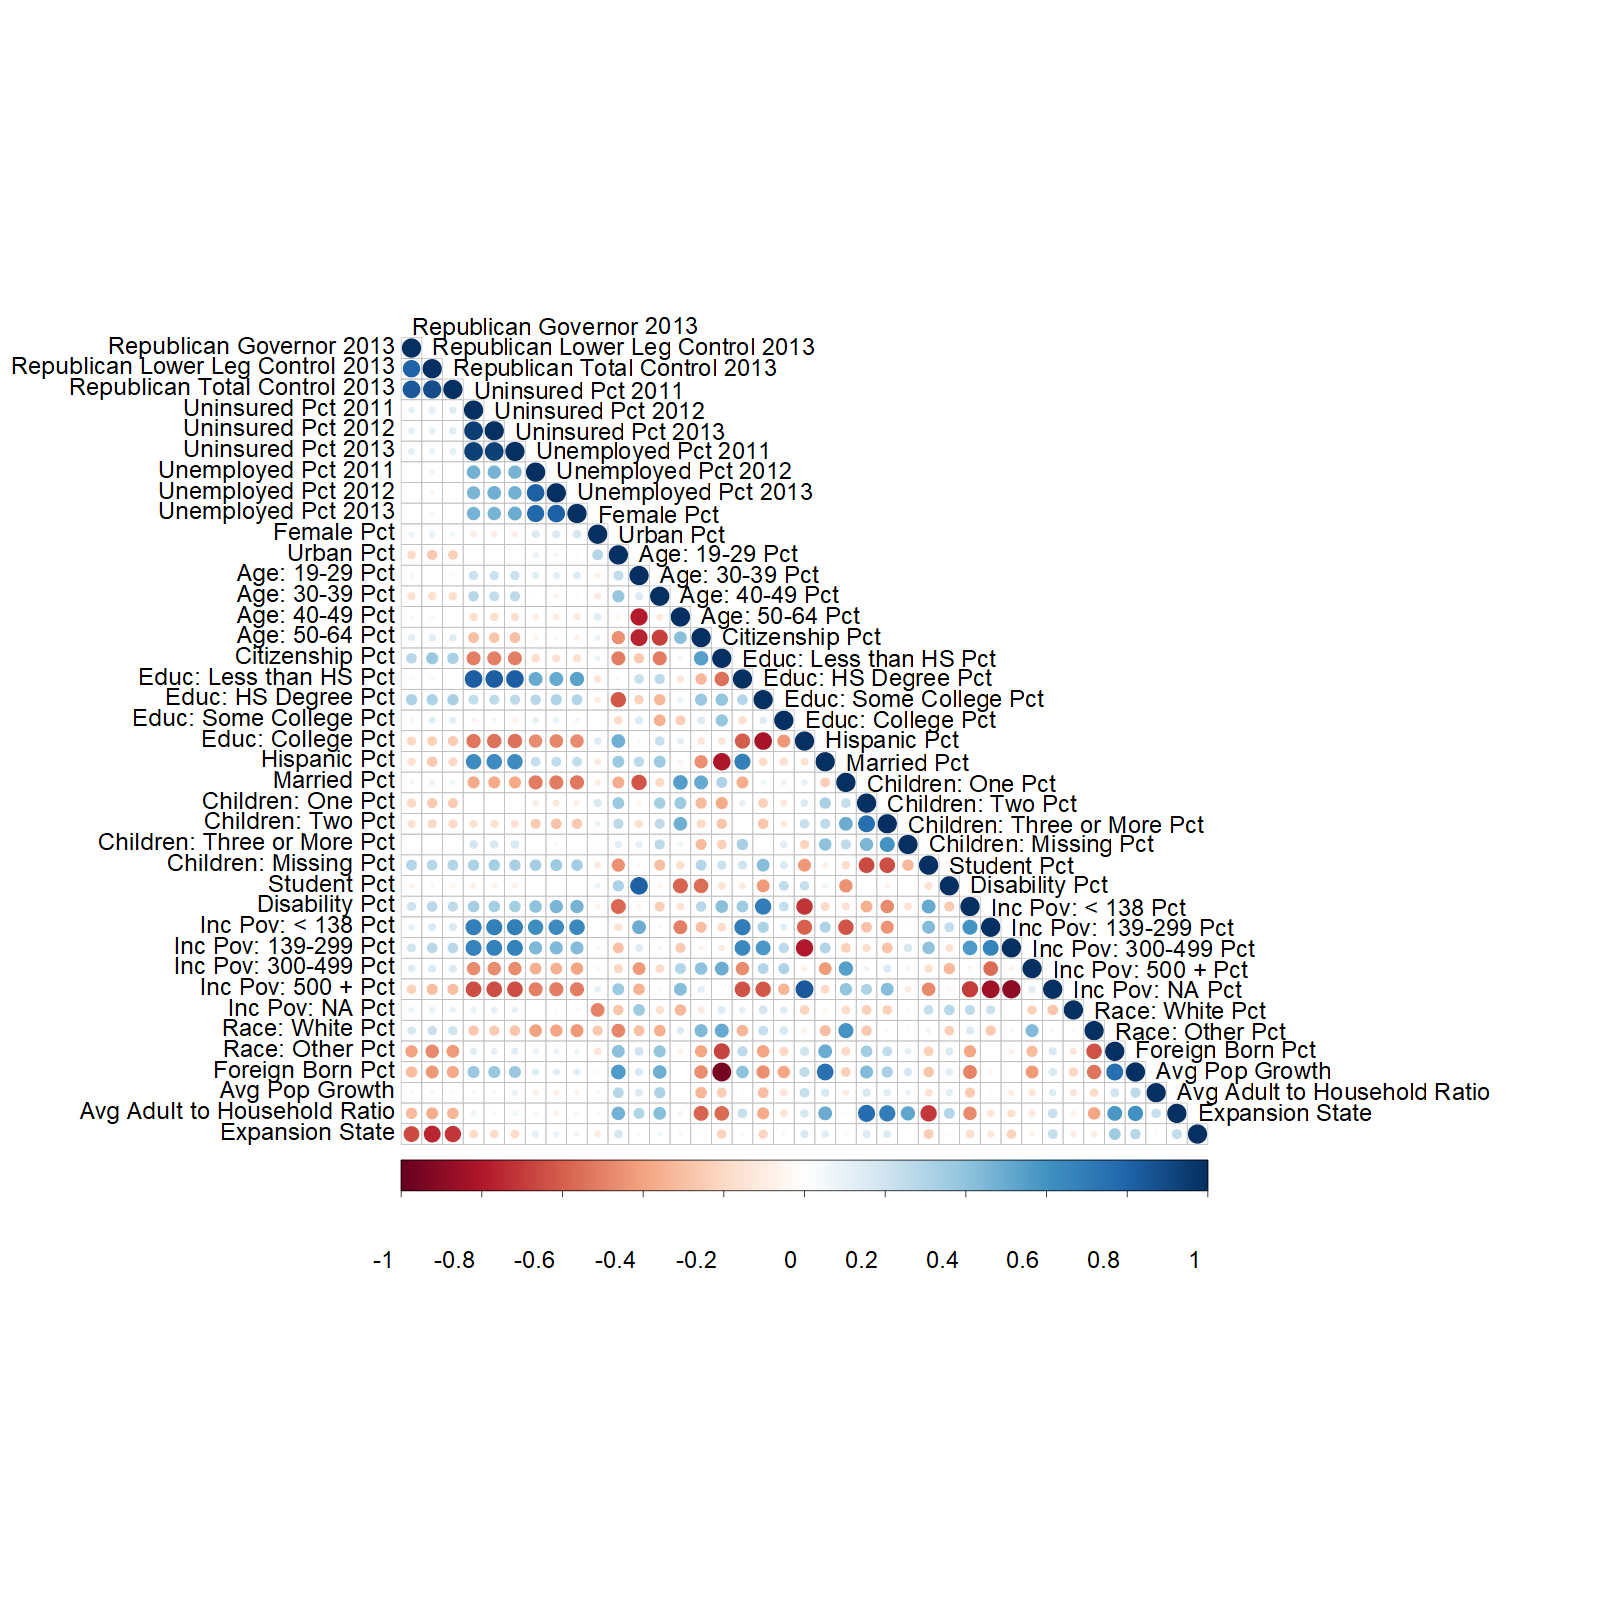
\includegraphics[scale=0.6]{01_Plots/correlation-plot-c1-sigma-zero.png}
\end{center}
\end{figure}
